\section{引言}

Julia 集是一种在复平面上非发散点形成的分形点的集合,由法国数学家 Gaston Maurice Julia 等人所提出。同 Mandelbrot 集一样,它可以由复数域下的简单多项式迭代而来,图像奇异美妙,又具有一定的几何规则。

几何学与人类文明如影随形。从古典的欧式几何到 Mandelbrot 提出的分形理论,在数学家们的眼中,具象的现实世界所刻画的纷繁形态似乎总是可以被抽象为简练的数学语言。

1967年,Mandelbrot 在研究海岸线长度时提出自然界中总是普遍存在着“自相似”的结构,并将此种整体与局部以某种方式相似的形体称作“分形”(Fractal),由此建立了一套未来将广泛用于工程、经济等各个领域的崭新理论。\textsuperscript{\cite{enwiki-mandelbortset}}作为迭代理论和现代分形理论的两位主要发明者之一, Julia 在研究复数多项式函数迭代的过程中意识到,随着迭代的进行,趋向于限制位置的点和从未稳定下来的点之间存在关键的区别,而后者便属于迭代的 Julia 集。\textsuperscript{\cite{website-julia}}

\begin{figure}[htbp]
\centering
\begin{minipage}{0.3\linewidth}
\centering
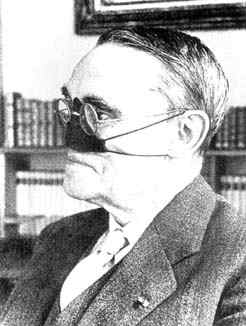
\includegraphics[width = 2.97cm]{./images/julia.jpg}
\caption{Gaston Maurice Julia\textsuperscript{\cite{pic-julia}}}
\label{fig1-1}
\end{minipage}\hfill
\begin{minipage}{0.3\linewidth}
\centering
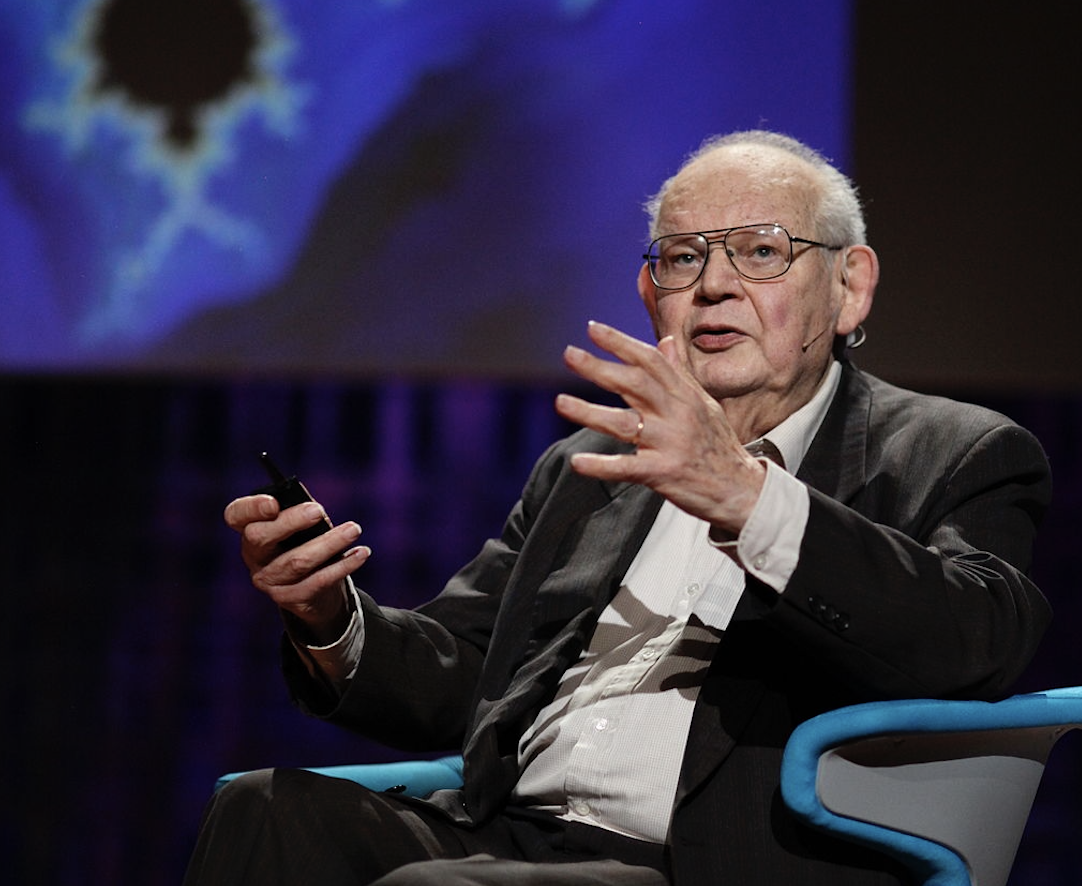
\includegraphics[width = 4.73cm]{./images/mandelbort.png}
\caption{Benoit B. Mandelbrot\textsuperscript{\cite{enwiki-mandelbort}}}
\label{fig1-2}
\end{minipage}\hfill
\begin{minipage}{0.35\linewidth}
\centering
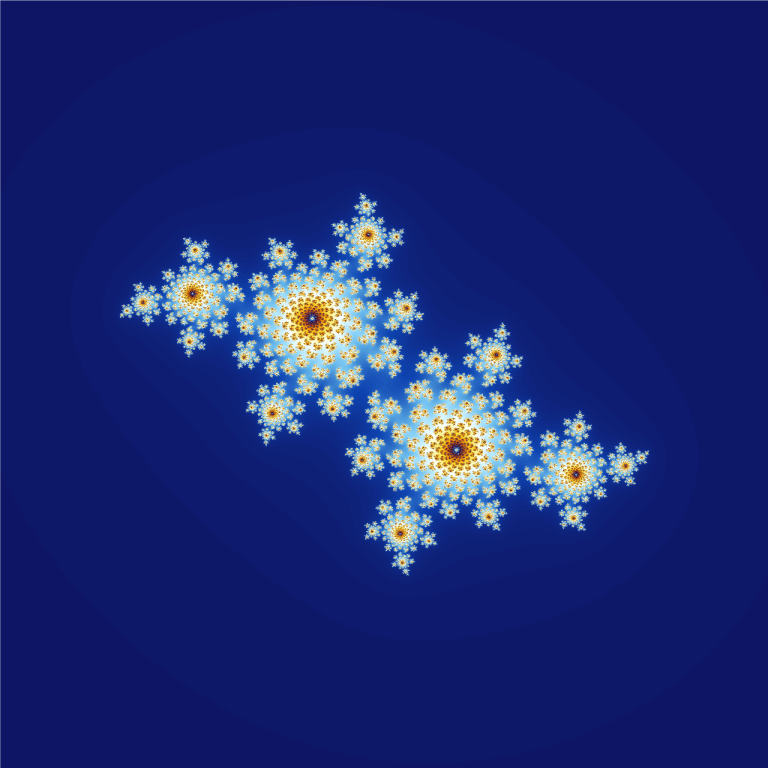
\includegraphics[width = 3.85cm]{./images/julia_set_example.png}
\caption{Julia 集:$c=−0.4+0.6i$\textsuperscript{\cite{enwiki-juliaset}}}
\label{fig1-3}
\end{minipage}
\end{figure}

只需利用最简单的迭代关系便能绘制出一幅极为规整复杂的图案,这是二者的精妙所在。本文将从 Julia 集出发,在分析其特性与算法的基础上,通过实例展现二者的内在联系与重要意义。